\documentclass[../../main.tex]{subfiles}

\graphicspath{{\subfix{../../immagini/}}}

\begin{document}

Le architetture di reti introdotte negli scorsi paragrafi risultano limitate in contesti in cui lavoro su dati che non sono indipendenti tra loro, come ad esempio sequenze di testo, in cui il significato di una parola può dipendere dal contesto in cui è inserita e di conseguenza dalle parole che la precedono: utilizzare una rete feedforward in un contesto del genere sarebbe limitante sia perchè la rete lavorerebbe solamente su sequenze di una lunghezza prefissata, sia perché ogni elemento in ingresso verrebbe considerato indipendente dai precedenti.

Quando ci si trova a lavorare con sequenze in cui ogni elemento risulta dipendente dai precedenti vengono spesso utilizzate le \textit{reti ricorrenti} (RNN). In reti di questo tipo è presente una corrispondenza uno a uno tra gli strati del modello ed il numero di elementi della sequenza, ciò permette quindi di avere in ingresso sequenze di lunghezze arbitraria; gli strati del modello inoltre \textit{condividono} gli stessi parametri, questo, oltre a portare ad un numero di parametri prefissato e non dipendente dalla lunghezze della sequenza, permette anche di dare importanza alla posizione, spesso chiamata \textit{timestamp}, di un elemento. La condivisione dei parametri viene concretizzata in questo modo: ogni risultato in uscita alla rete è funzione dei risultato prodotti in uscita negli istanti precedenti, e ogni risultato viene calcolato utilizzando la stessa regola di aggiornamento applicata ai precedenti risultati.

Per rappresentare una rete ricorrente è utile introdurre il concetto di \textit{grafo computazionale}: in un grafo di questo tipo ogni nodo indica una variabile, che può essere una scalare, un vettore, una matrice $\dots$ mentre un arco $(x,y)$ indica l'utilizzo della variabile $x$ in una \textit{operazione} che ha come risultato $y$.\\
Un grafo computazionale viene definito con una serie di operazioni base, operazioni più complesse vengono rappresentate come combinazioni di quelle base.

Formalmente posso rappresentare lo stato di un livelo nascosto della rete ricorrente come:
\[\boldsymbol{h}^{(t)} = f(\boldsymbol{h}^{(t-1)}, \boldsymbol{x}^{(t)}; \boldsymbol{\Theta})\]
in questo caso $\boldsymbol{h}$ rappresenta lo stato del livello al tempo $t$ (Da non confondere con $h$ funzione d'ipotesi).\\
Posso rappresentare questa funzione ricorsiva tramite il grafo computazionale in Figura \ref{fig:computationgraph}.
\begin{figure}[H]
    \centering
    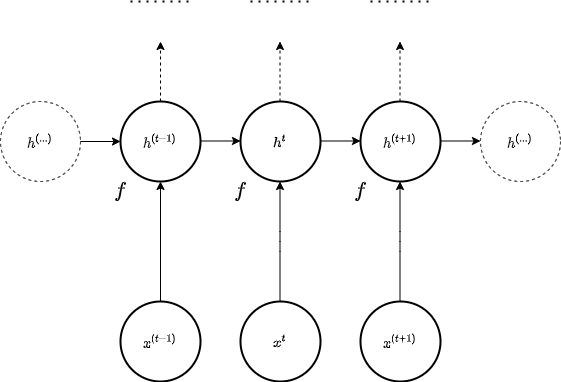
\includegraphics[scale = 0.4]{immagini/4_2/computation_graph.png}
    \caption{}
    \label{fig:computationgraph}
\end{figure}
Il grafo mostra inoltre come un singolo modello possa lavorare su sequenze di lunghezza arbitraria, permettendo di fornire risultati anche su sequenze di lunghezze diverse  da quelle presenti nel dataset d'addestramento.

Come accade nelle reti feedforward anche in questo caso, definite le caratteristiche base di una rete ricorrente, posso combinare gli elementi a disposizione per andare a creare diverse architetture, alcune delle più frequenti sono:

\begin{itemize}
    \item Reti ricorrenti che producono un risultato ad ogni istante di tempo ed hanno connessioni ricorrenti tra strati nascosti. (Figura \ref{fig:RNNArch1})
    \item Reti ricorrenti che producono un risultato ad ogni istante di tempo ed hanno connessioni tra il risultato al tempo $t-1$ e lo strato nascosto al tempo $t$. (Figura \ref{fig:RNNArch2})
    \item Reti ricorrenti con connessioni tra strati nascosti e che producono un solo risultato al termine della sequenza. (Figura \ref{fig:RNNArch3})
\end{itemize}

\begin{figure}[H]
    \centering
    \begin{subfigure}[t]{0.49\textwidth}
        \centering
        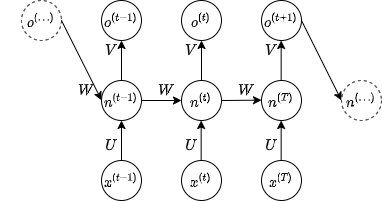
\includegraphics[width = \textwidth]{immagini/4_2/recnet.png}
        \caption{RNN con uscita ad ogni istante di tempo}
        \label{fig:RNNArch1}
    \end{subfigure}
    \begin{subfigure}[t]{0.49\textwidth}
        \centering
        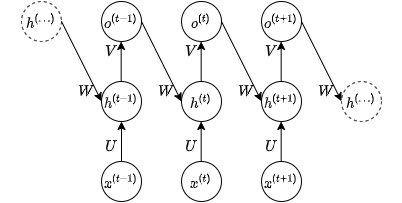
\includegraphics[width = \textwidth]{immagini/4_2/recnet2.png}      
        \caption{RNN in cui l'uscita di ogni istante di tempo influenza lo strato nascosto dell'istante successivo}  
        \label{fig:RNNArch2}
    \end{subfigure}
    \begin{subfigure}[t]{0.49\textwidth}
        \centering
        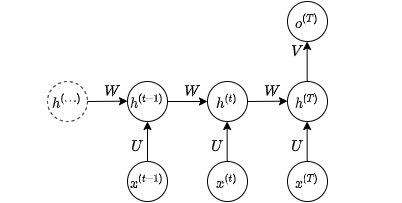
\includegraphics[width = \textwidth]{immagini/4_2/recnet3.png}  
        \caption{RNN con uscita solo all'ultimo istante di tempo} 
        \label{fig:RNNArch3}  
    \end{subfigure}
\end{figure}

Nel corso del tempo sono state proposte diverse implementazioni di questo tipo di architetture, quella da noi utilizzata negli esperimenti prende il nome di \textit{Gated Recurrent Unit} (GRU), la sua struttura viene introdotta nei paragrafi successivi.

\subsubsection{Apprendimento nelle reti ricorrenti}
Anche le RNN rientrano nella tipologia di modelli parametreci, l'apprendimento quindi avviene anche in questo caso cercando il miglior insieme di parametri sulla base degli elementi del training set; l'algoritmo più spesso utilizzato è ancora una volta la discesa del gradiente.

Per il calcolo del gradiente viene sfruttata una variante della  backpropagation, chiamata \textit{backpropagation through time} (BPTT), usata per far fronte ai problemi che sorgono dalla convisione dei parametri; prima di introdurre la BPTT definisco le equazioni che descrivono la \textit{forward propagation} degli elementi in ingresso alla rete: il primo passo è l'inizializzazione dello strato nascosto al tempo 0 $\boldsymbol{h}^{(0)}$, successivamente ad ogni istante di tempo il risultato delle rete viene calcolato come:
\begin{fleqn}[1cm]
    \begin{equation}
        \boldsymbol{a}^{(t)} = \boldsymbol{b} + \boldsymbol{W h}^{t-1} + \boldsymbol{U x}^{(t)}
    \end{equation}
    \begin{equation}
        \boldsymbol{h}^{(t)} = tanh(\boldsymbol{a}^{(t)})
    \end{equation}
    \begin{equation}
        \boldsymbol{o}^{(t)} = \boldsymbol{c} + \boldsymbol{V h}^{(t)}
    \end{equation}
    \begin{equation}
        \boldsymbol{\hat{y}}^{(t)} = softmax(\boldsymbol{o}^{(t)})
    \end{equation}
\end{fleqn}
Suppongo quindi che la funzione di attivazione utilizzata sia una tangente iperbolica (\textit{tanh}) e che il vettore dei risultati in un generico istante $\boldsymbol{\hat{y}}^{(t)}$ sia ottenuto applicando una funzione softmax ai risultati della rete, di fatto ottenendo un vettore di probabilità; infine i parametri $\boldsymbol{U}$, $\boldsymbol{V}$ e $\boldsymbol{W}$ rappresentano le matrici di pesi rispettivamente tra livello d'ingresso e nascosto, livello nascosto e output e livello nascosto e livello nascosto all'istante successivo, $\boldsymbol{b}$ e $\boldsymbol{c}$ rappresentano invece i vettori di bias.

In questo caso inoltre utilizzo la funzione di \textit{log-verosimiglianza} come misura dell'errore commesso dal modello, in un generico istante $t$ quindi misuro la perdita come:
\[L^{(t)} = -\log(\boldsymbol{y}^{(t)}) = -\log(softmax(\boldsymbol{o}^{(t)}))\]
Mentre la perdita totale per una data sequenza $\boldsymbol{x}$ è data semplicemente dalla somma delle perdite nei singoli istanti:
\[L = \sum_t L^{(t)}\]
Per il calcolo del gradiente (Sfruttato poi per l'aggiornamento dei pesi) si ricorre anche in questo caso alla \textit{retropropagazione}, la caratteristica delle reti ricorrenti di avere pesi condivisi obbliga però a variare leggermente l'approccio base, adottato nei percettroni multistrato, questa variante dell'algoritmo prende il nome di \textit{backpropagation through time (BPTT)}.
 
Il primo passo consiste nel calcolare i gradienti $\nabla_{\boldsymbol{N}}L$ dei nodi $\boldsymbol{N}$ interni del grafo computazionale:
\begin{fleqn}[1cm]
    \begin{align}
        \frac{\partial L}{\partial L ^ {(t)}} = \frac{\partial}{\partial L ^{(t)}} \sum_t L^{(t)} = 1
    \end{align}
    \begin{align}
        (\nabla_{\boldsymbol{o}^{(t)}}L)_i = \frac{\partial L}{\partial o^{(t)}_i} = \frac{\partial L}{\partial L^{(t)}} \frac{\partial L^{(t)}}{\partial o^{(t)}_i} = 1 \cdot (\hat{y_i}^{(t)} - 1_{i,y^{(t)}})
        \label{eqn:BPTT}
    \end{align}
    \begin{align}
        \nabla_{\boldsymbol{h}^{(t)}}L = \left(\frac{\partial \boldsymbol{h}^{(t+1)}}{\partial \boldsymbol{h}^{(t)}}\right)^T (\nabla_{\boldsymbol{h}^{(t+1)}}L) + \left(\frac{\partial \boldsymbol{o}^{(t)}}{\partial \boldsymbol{h}^{t}}\right)^T (\nabla_{\boldsymbol{o}^{(t)}}L)
    \end{align}
    \begin{align}
        \nabla_{\boldsymbol{h}^{(\mathcal{T})}}L = \boldsymbol{V}^T \nabla_{\boldsymbol{o}^{(\mathcal{T})}} L 
    \end{align}
\end{fleqn}
Dove il risultato dell'equazione \ref{eqn:BPTT} viene giustificato ricordando come la funzione di perdita è definita e applicando la \textit{regola della catena}:
\[- \frac{\partial}{\partial o_i^{(t)}} \log(\hat{y}^{(t)}) = - \left(\frac{\partial \log(\hat{y}_i^{(t)})}{\partial \hat{y}_i^{(t)}} \cdot\frac{\partial softmax(o_i^{(t)})}{\partial o_i^{(t)}}\right) = \cdots = \hat{y_i}^{(t)} - 1_{i,y^{(t)}}\]
Sfruttando ancora una volta la regola della catena ed i risultati appena ottenuti posso ricavare i gradienti dei \textit{parametri} del grafo:

\begin{fleqn}[1cm]
    \begin{align}
        \nabla_{\boldsymbol{V}}L = \sum_t \sum_i \left(\frac{\partial L}{\partial o_i^{(t)}}\right) \nabla_{\boldsymbol{V}}o_i^{(t)} = \sum_t (\nabla_{o^{(t)}}L) \boldsymbol{h}^{(t)^T}
    \end{align}
    \begin{align}
        \nabla_{\boldsymbol{W}}L = \sum_t \sum_i \frac{\partial L}{\partial h_i^{(t)}} \nabla_{\boldsymbol{W^{(t)}}} h_i^{(t)} = \sum_t \text{diag} \left(1 - (\boldsymbol{h^{(t)}})^2\right) (\nabla_{\boldsymbol{h}^{(t)}}L)\boldsymbol{h}^{(t-1)^T}
    \end{align}
    \begin{align}
        \nabla_{\boldsymbol{U}}L = \sum_t \sum_i \left(\frac{\partial L}{\partial h_i^{(t)}}\right) \nabla_{\boldsymbol{U}^{(t)}}h_i^{(t)} = \sum_t \text{diag} \left(1 - (\boldsymbol{h^{(t)}})^2\right) (\nabla_{\boldsymbol{h}^{(t)}}L )\boldsymbol{x}^{(t)^T}
    \end{align}
    \begin{align}
        \nabla_{\boldsymbol{c}}L = \sum_t \left(\frac{\partial \boldsymbol{o}^{(t)}}{\partial \boldsymbol{c}}\right)^T \nabla_{(\boldsymbol{o}^{(t)})}L = \sum_t \nabla_{\boldsymbol{o}^{(T)}} L
    \end{align}
    \begin{align}
        \nabla_{\boldsymbol{b}}L = \sum_t \left(\frac{\partial \boldsymbol{h}^{(t)}}{\partial \boldsymbol{b}^{(t)}}\right)^T \nabla_{\boldsymbol{h}^{(t)}} L = \sum_t \text{diag}\left(1 - (\boldsymbol{h}^{(t)})^2\right)\nabla_{\boldsymbol{h}^{(t)}}L
    \end{align}
\end{fleqn}
Dove $\text{diag} \left(1 - (\boldsymbol{h^{(t)}})^2\right)$ indica la matrice diagonale contenente gli elementi $1 - (\boldsymbol{h^{(t)}})^2$ e corrisponde di fatto alla matrice delle derivate parziali della tangente iperbolica.\\
La notazione $\boldsymbol{W}^{(T)}$ indica il contributo della matrice di pesi al tempo $t$, in altre parole sto supponendo che i parametri tra uno strato nascosto e quello temporalmente successivo siano indipendenti tra loro, ciò mi permette di calcolare il contributo dei pesi in ogni istante di tempo per poi sommare tali contributi ottenendo il gradiente totale da utilizzare poi per l'aggiornamento.
\end{document}